% Tdyssey talk (10 minutes). Build from this folder: pdflatex main.tex (twice), or upload presentation/ to Overleaf
% and set slides/main.tex as the main file. Figures: ../figures (PDF), images: ../images, video stills: ../videos/posters.
% Videos open in the system player when their still is clicked (keep the videos/ folder next to slides/).
\documentclass[aspectratio=169,11pt]{beamer}
\usepackage[T1]{fontenc}
\usepackage{lmodern}
\usepackage{graphicx}
\usepackage{booktabs}
\usepackage{tikz}
\usetikzlibrary{arrows.meta,positioning,calc}
\graphicspath{{../figures/}{../images/}{../videos/posters/}}

% ---- look: plain, readable from the back of the room
\usetheme{default}
\setbeamertemplate{navigation symbols}{}
\setbeamertemplate{footline}[frame number]
\definecolor{tdblue}{HTML}{2A78D6}
\definecolor{tdgrey}{HTML}{6B6B6B}
\definecolor{tdorange}{HTML}{EB6834}
\setbeamercolor{frametitle}{fg=tdblue}
\setbeamercolor{title}{fg=tdblue}
\setbeamercolor{itemize item}{fg=tdblue}
\setbeamerfont{frametitle}{series=\bfseries}

% \video{still image}{video path relative to slides/}{width}: a still that opens the video when clicked
\newcommand{\video}[3]{\href{run:#2}{\includegraphics[width=#3]{#1}}}
\newcommand{\note}[1]{{\footnotesize\color{tdgrey}#1}}

\title{Tdyssey: one camera policy for every letter}
\subtitle{Adapting a T-only Diffusion Policy to 26 letters without new human demonstrations}
\author{Tdyssey team} % TODO: author names
\institute{CS5478}
\date{}

\begin{document}

\begin{frame}
  \titlepage
  \vspace{-1.2em}
  \centering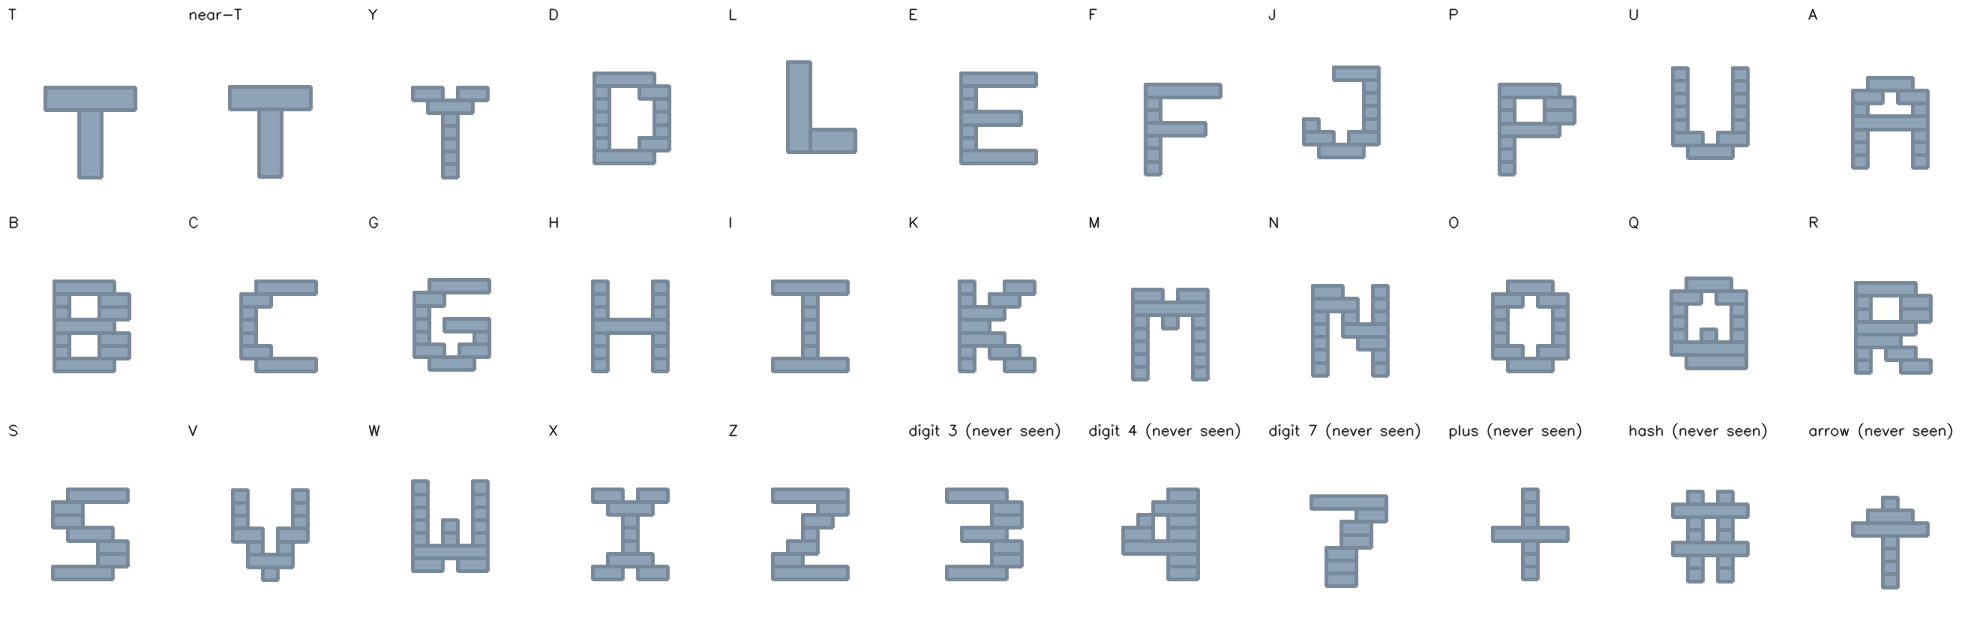
\includegraphics[width=0.92\textwidth]{shape_gallery_33_upright.png}
\end{frame}

% ------------------------------------------------------------------ 1. problem
\begin{frame}{The problem: a policy that only knows the T}
  \begin{columns}[T]
    \column{0.48\textwidth}
    \video{compare_P.png}{../videos/compare/P.mp4}{\linewidth}\\
    \note{Same scene: original policy (left) and ours (right). Click to play.}
    \column{0.5\textwidth}
    \begin{itemize}
      \item Official RSS 2023 camera Diffusion Policy for PushT: push a block onto a goal outline.
      \item Trained on human demonstrations of the \textbf{T only}.
      \item On the other 26 shapes it succeeds \textbf{3.7\%} of the time.
      \item Goal: \textbf{one} policy for all 26 capital letters and near-T, \textbf{without} new human demonstrations.
    \end{itemize}
  \end{columns}
\end{frame}

\begin{frame}{Rules we set ourselves}
  \centering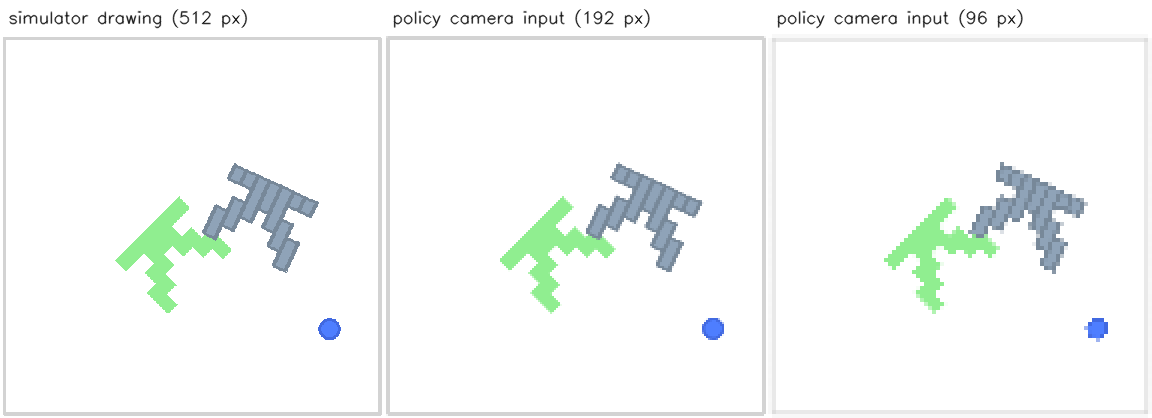
\includegraphics[width=0.9\textwidth]{camera_views_512_192_96.png}
  \begin{itemize}
    \item The deployed policy sees only the camera image (96$\times$96, as the original) and the pusher position.
    \item Exact simulator state may be used \emph{only} to make training data, and is disclosed.
    \item Every claim is tested on fresh scenes, fixed in advance, with all policies on the same scenes.
  \end{itemize}
\end{frame}

% ------------------------------------------------------------------ 2. what did not work
\begin{frame}{First attempt: reinforcement learning in the simulator}
  \begin{columns}[T]
    \column{0.5\textwidth}
    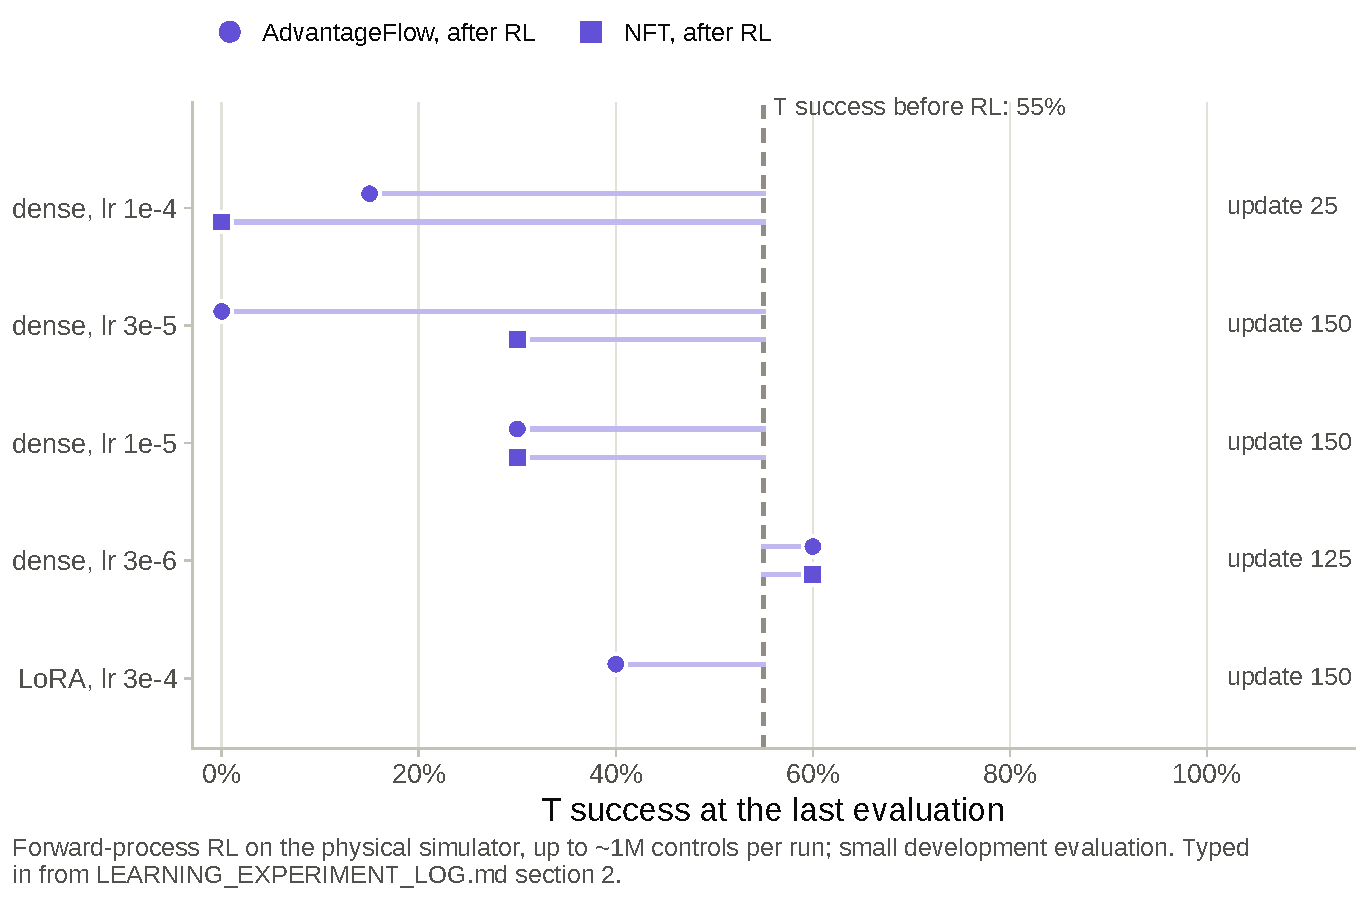
\includegraphics[width=\linewidth]{rl_t_collapse.pdf}
    \column{0.5\textwidth}
    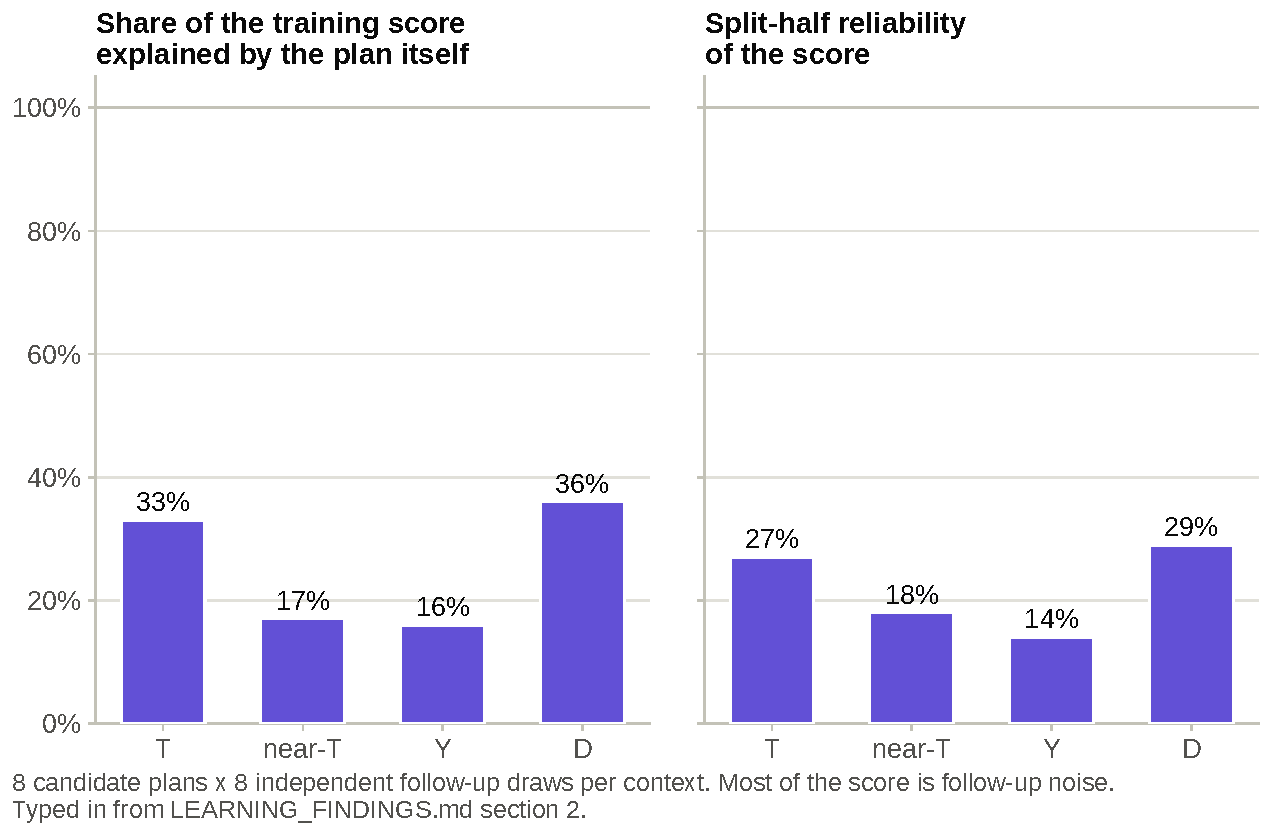
\includegraphics[width=\linewidth]{rl_signal_variance.pdf}
  \end{columns}
  \begin{itemize}
    \item Small steps changed nothing; larger steps destroyed the T skill.
    \item The training score was mostly noise: only 16--36\% of it came from the plan being scored.
  \end{itemize}
\end{frame}

% ------------------------------------------------------------------ 3. method
\begin{frame}{The teacher: plan inside a learned world model}
  \begin{columns}[T]
    \column{0.48\textwidth}
    \video{teacher_9shapes.png}{../videos/teacher/teacher_9shapes.mp4}{\linewidth}\\
    \note{Red dot: next push; pink: rest of the planned path.}
    \column{0.5\textwidth}
    \begin{itemize}
      \item World model of the pushing physics, learned from non-expert machine rollouts.
      \item Planner tries about 1{,}150 candidate pushes per step inside it.
      \item Reads exact block and pusher positions: a \textbf{teacher}, not a deployable policy.
    \end{itemize}
    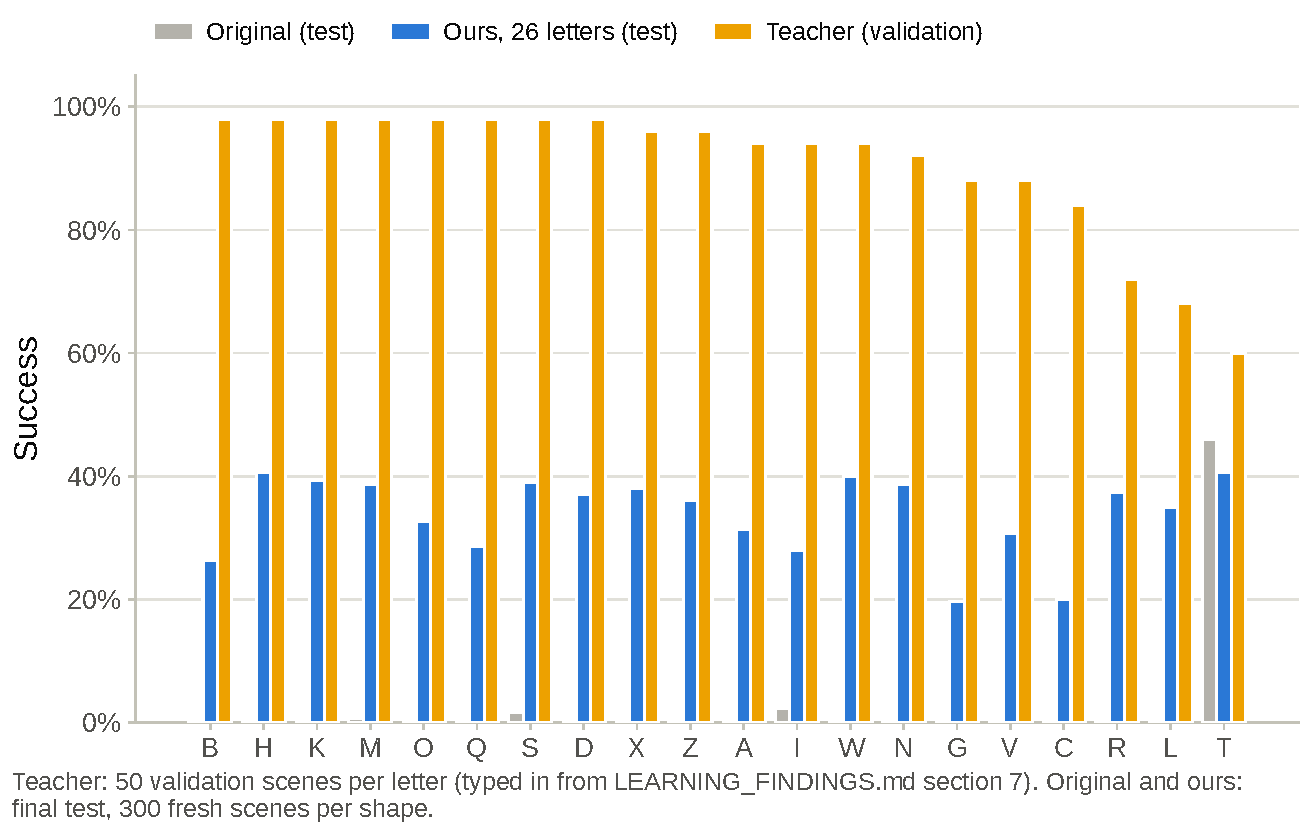
\includegraphics[width=\linewidth]{method_teacher_success_26letters.pdf}
  \end{columns}
\end{frame}

\begin{frame}{From teacher to camera policy}
  \centering
  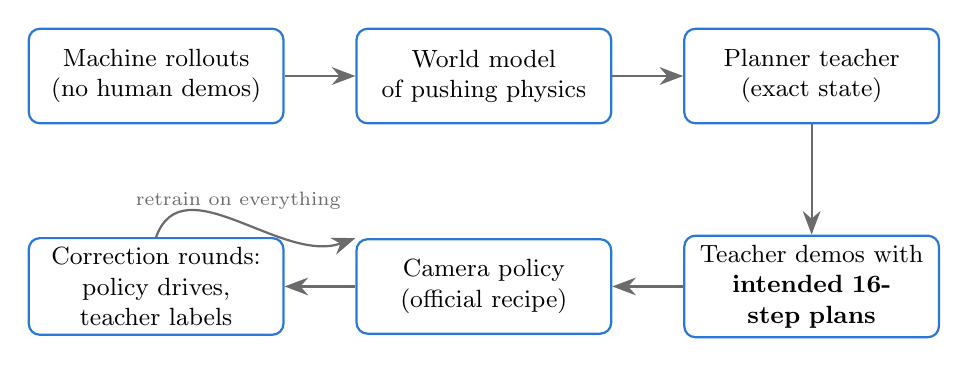
\begin{tikzpicture}[node distance=7mm and 9mm, box/.style={draw=tdblue, rounded corners, thick, align=center,
      minimum height=12mm, text width=30mm, font=\small}, arr/.style={-{Stealth[length=3mm]}, thick, tdgrey}]
    \node[box] (data) {Machine rollouts\\(no human demos)};
    \node[box, right=of data] (wm) {World model\\of pushing physics};
    \node[box, right=of wm] (teacher) {Planner teacher\\(exact state)};
    \node[box, below=14mm of teacher] (demos) {Teacher demos with\\\textbf{intended 16-step plans}};
    \node[box, left=of demos] (student) {Camera policy\\(official recipe)};
    \node[box, left=of student] (rounds) {Correction rounds:\\policy drives,\\teacher labels};
    \draw[arr] (data) -- (wm); \draw[arr] (wm) -- (teacher); \draw[arr] (teacher) -- (demos);
    \draw[arr] (demos) -- (student); \draw[arr] (student) -- (rounds);
    \draw[arr] (rounds.north) to[out=70, in=200] node[above, font=\scriptsize, text=tdgrey] {retrain on everything} (student.north west);
  \end{tikzpicture}
  \vspace{4mm}
  \begin{itemize}
    \item Labels: the teacher's \emph{intended} plan, not its executed pushes (129 vs 77 successes of 1000).
    \item Every training batch gives each shape an equal share; 54k steps and 60 practice scenes per new letter per round.
  \end{itemize}
\end{frame}

% ------------------------------------------------------------------ 4. results
\begin{frame}{Training: 5 $\rightarrow$ 10 $\rightarrow$ 27 shapes}
  \centering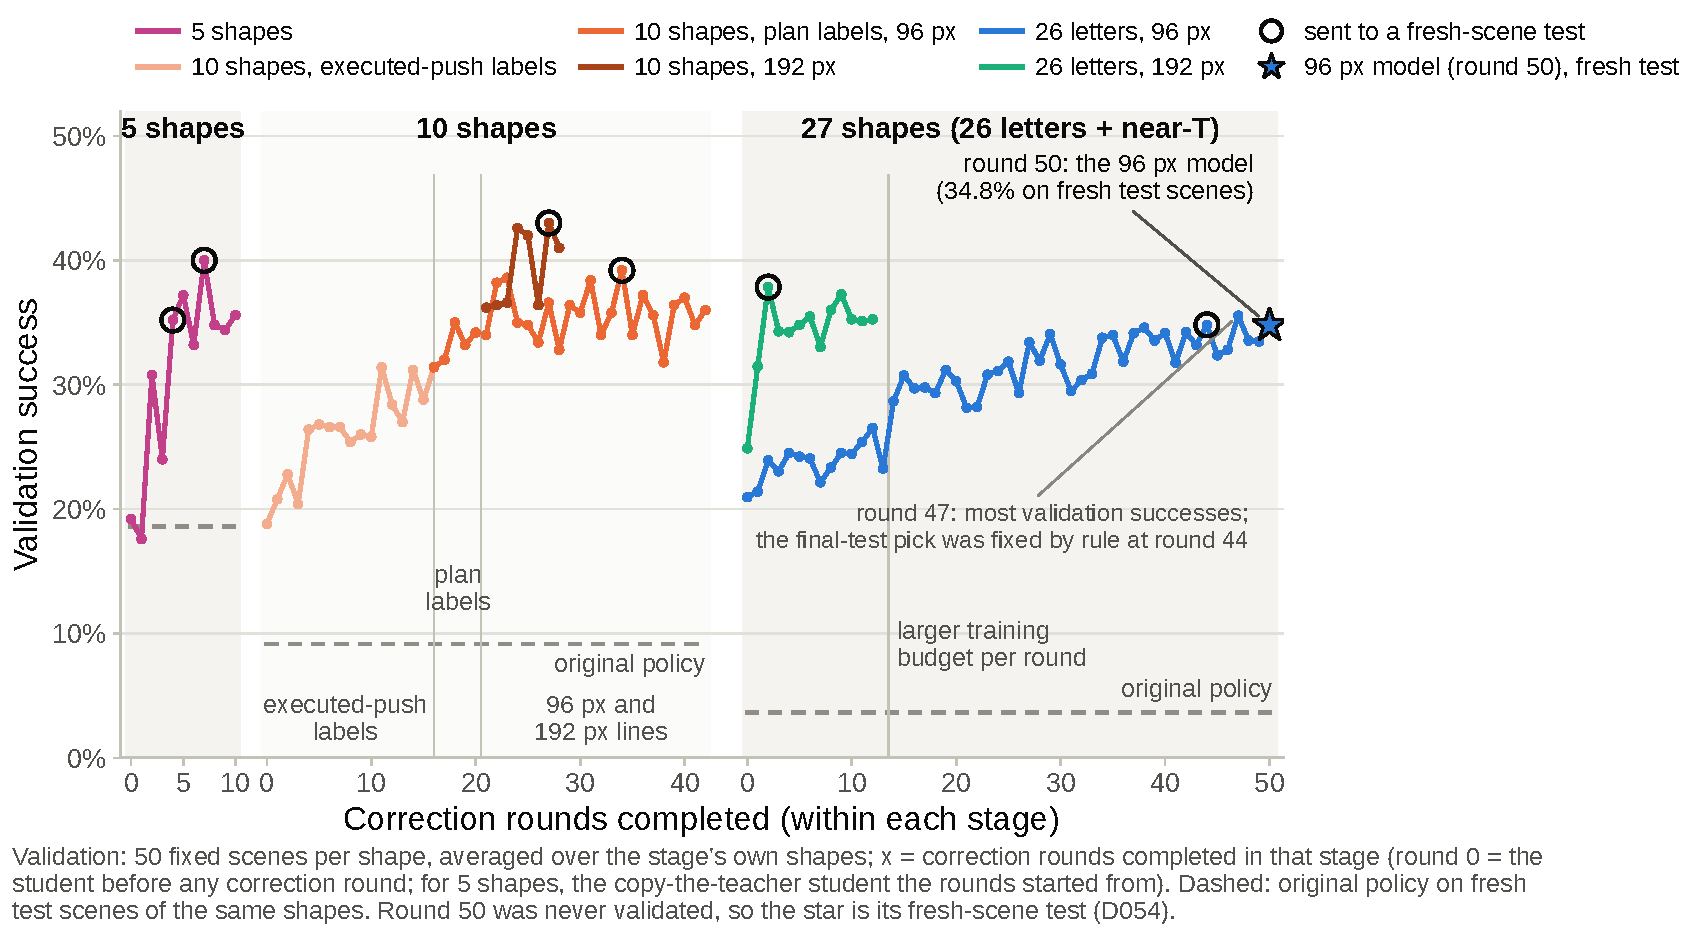
\includegraphics[width=0.95\textwidth]{curves_all_stages.pdf}
\end{frame}

\begin{frame}{26 letters: the per-shape budget was the bottleneck}
  \begin{columns}[T]
    \column{0.62\textwidth}
    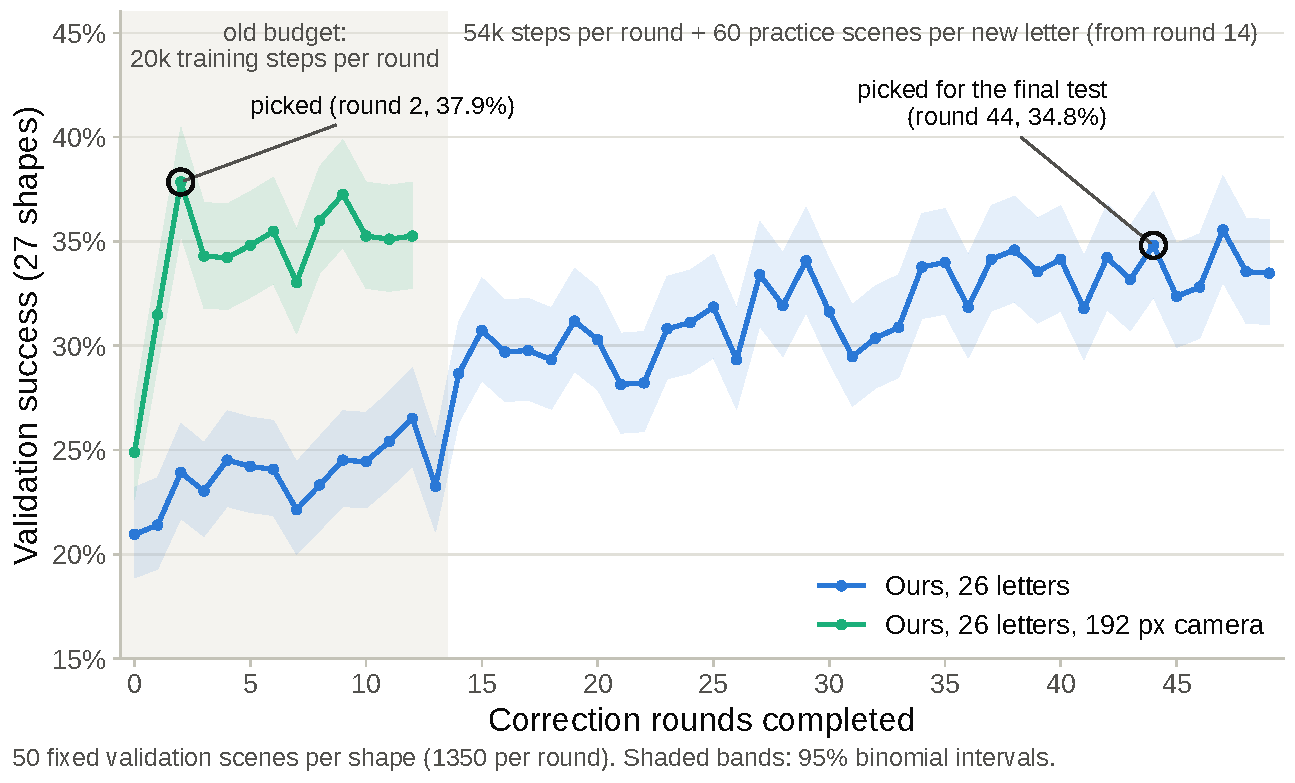
\includegraphics[width=\linewidth]{curves_26letters.pdf}
    \column{0.36\textwidth}
    \begin{itemize}
      \item 27 shapes sharing the 10-shape budget levelled off near 24\%.
      \item 54k steps per round and more practice scenes for new letters: about 35\%.
      \item The 17 new letters caught up with the 10 earlier shapes.
    \end{itemize}
  \end{columns}
\end{frame}

\begin{frame}{Final test: 300 fresh scenes per shape}
  \begin{columns}[T]
    \column{0.6\textwidth}
    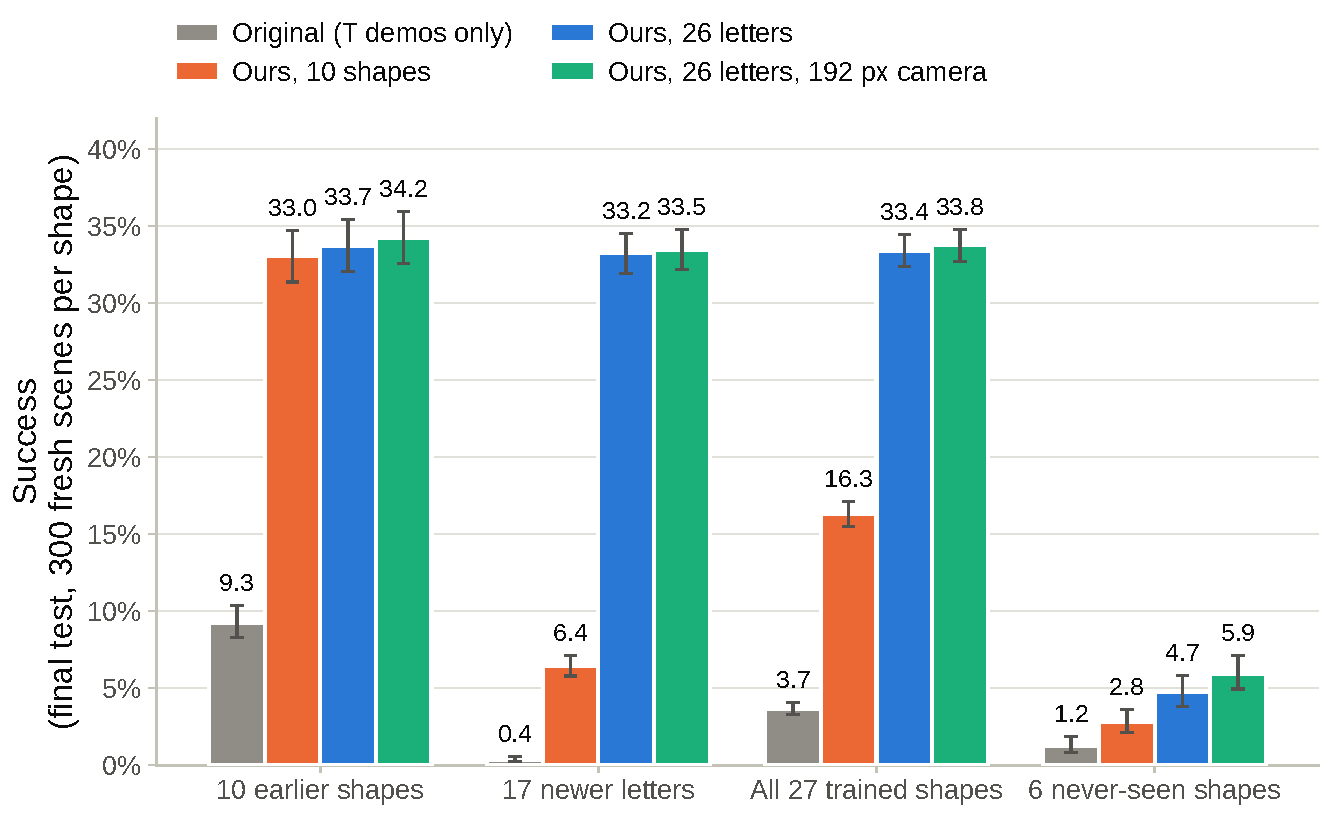
\includegraphics[width=\linewidth]{final_grouped_bars.pdf}
    \column{0.38\textwidth}
    \begin{itemize}
      \item 27 trained shapes: \textbf{3.7\% $\rightarrow$ 33.4\%} (96 px), 33.8\% (192 px).
      \item No loss on the ten earlier shapes when 17 letters were added.
      \item Six more rounds: 34.8\% (+1.9 points [+0.1, +3.6]).
      \item Goal covered at the end: 0.35 $\rightarrow$ 0.82.
    \end{itemize}
  \end{columns}
\end{frame}

\begin{frame}{Every shape improves}
  \centering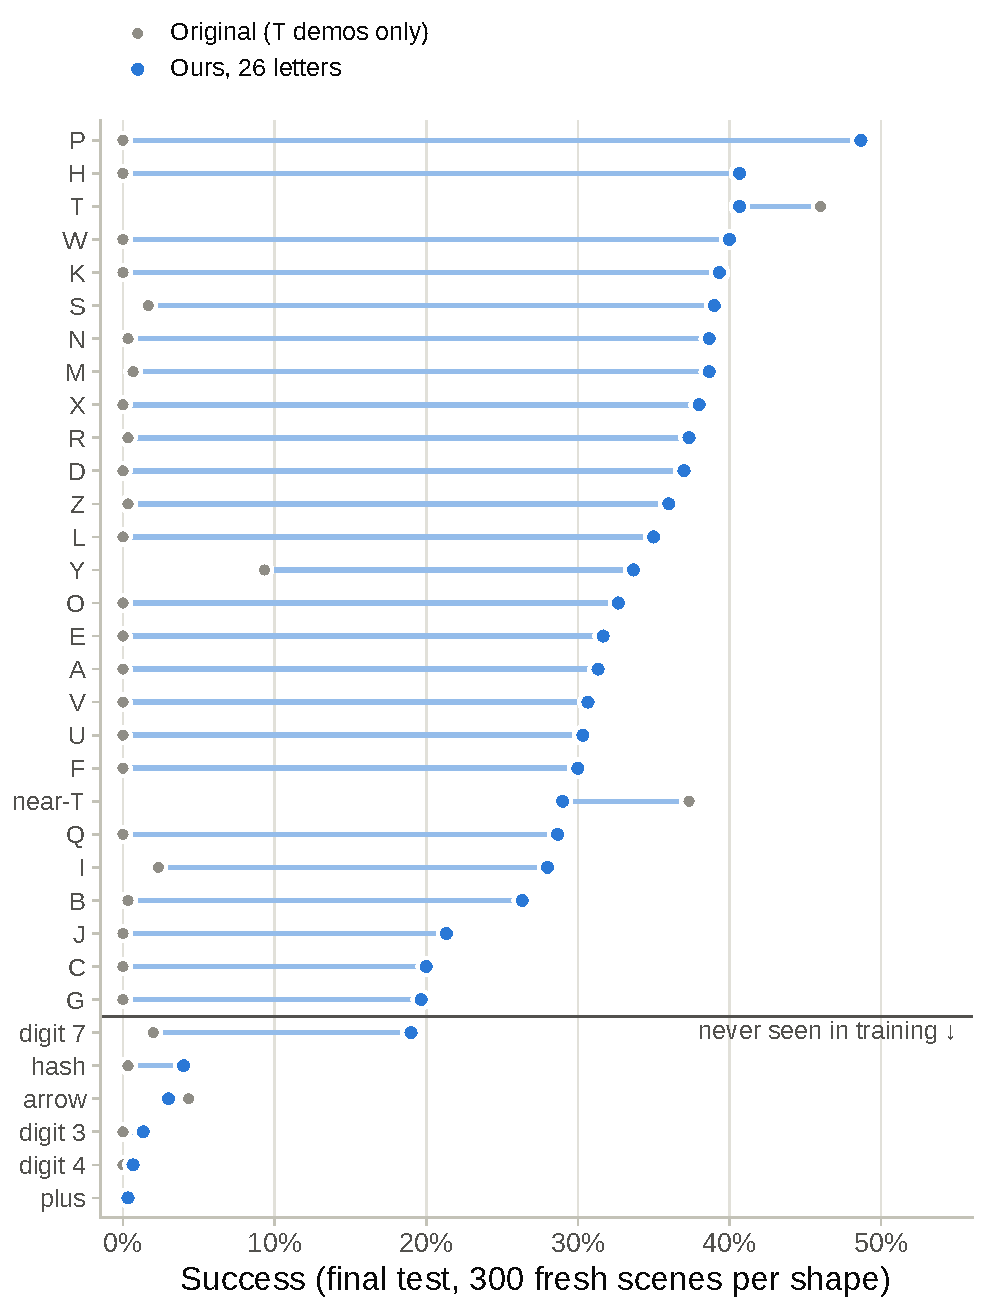
\includegraphics[height=0.82\textheight]{final_dumbbell.pdf}
\end{frame}

\begin{frame}{Demos: same scene, original vs ours}
  \begin{columns}[T]
    \column{0.32\textwidth}
    \video{compare_A.png}{../videos/compare/A.mp4}{\linewidth}
    \column{0.32\textwidth}
    \video{compare_M.png}{../videos/compare/M.mp4}{\linewidth}
    \column{0.32\textwidth}
    \video{compare_S_scene2.png}{../videos/compare/S_scene2.mp4}{\linewidth}
  \end{columns}
  \vspace{2mm}
  \centering\video{l26_r50_33shapes.png}{../videos/all_shapes/l26_r50_33shapes.mp4}{0.42\textwidth}\\
  \note{Examples where ours succeeds; it succeeds on about a third of scenes (failures: videos/failures/, list: videos/INDEX.md).}
\end{frame}

\begin{frame}{Never-seen shapes and the remaining gap}
  \begin{columns}[T]
    \column{0.5\textwidth}
    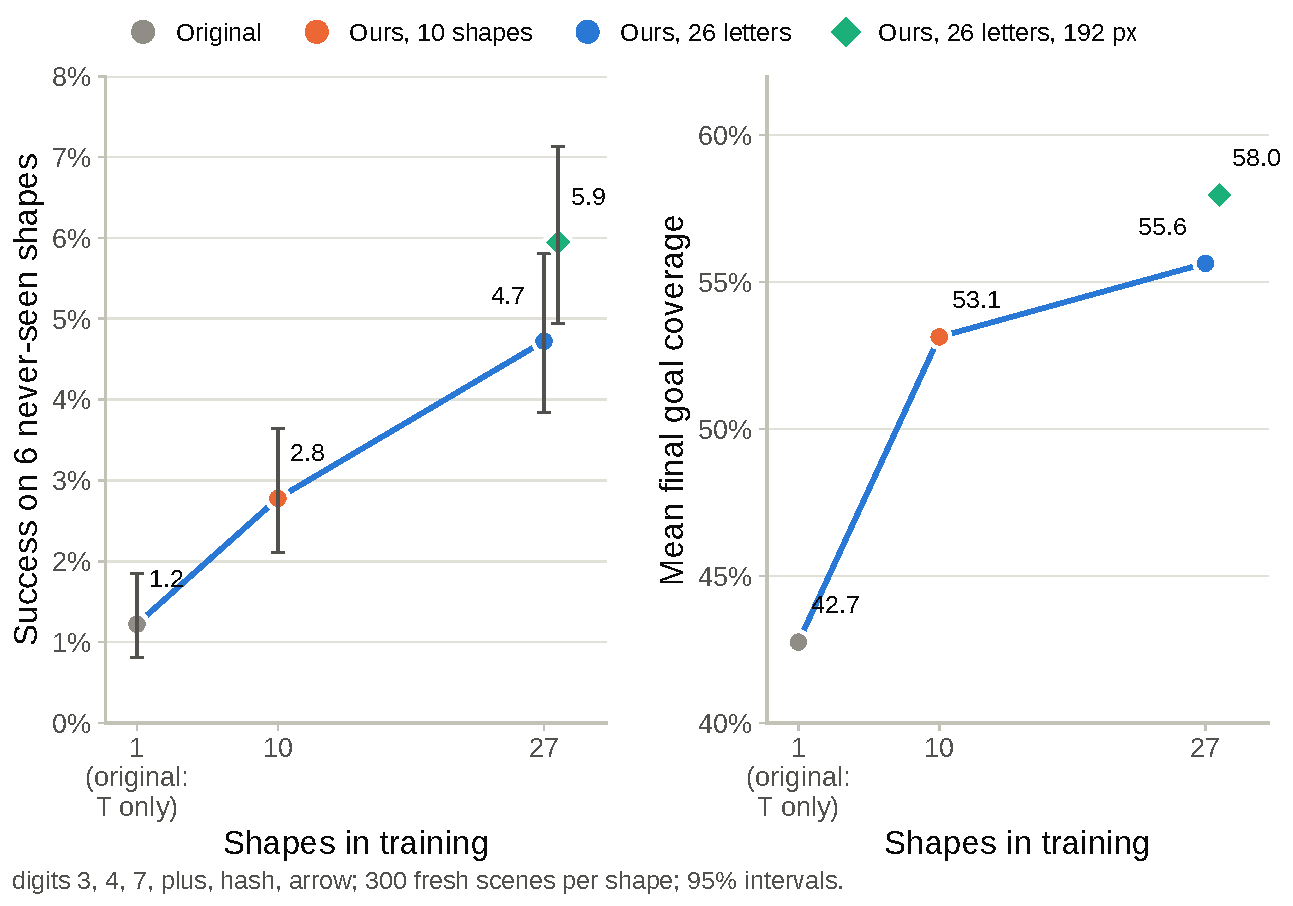
\includegraphics[width=\linewidth]{heldout_scaling.pdf}
    \note{Six shapes never used in training: success grows with the number of training shapes.}
    \column{0.5\textwidth}
    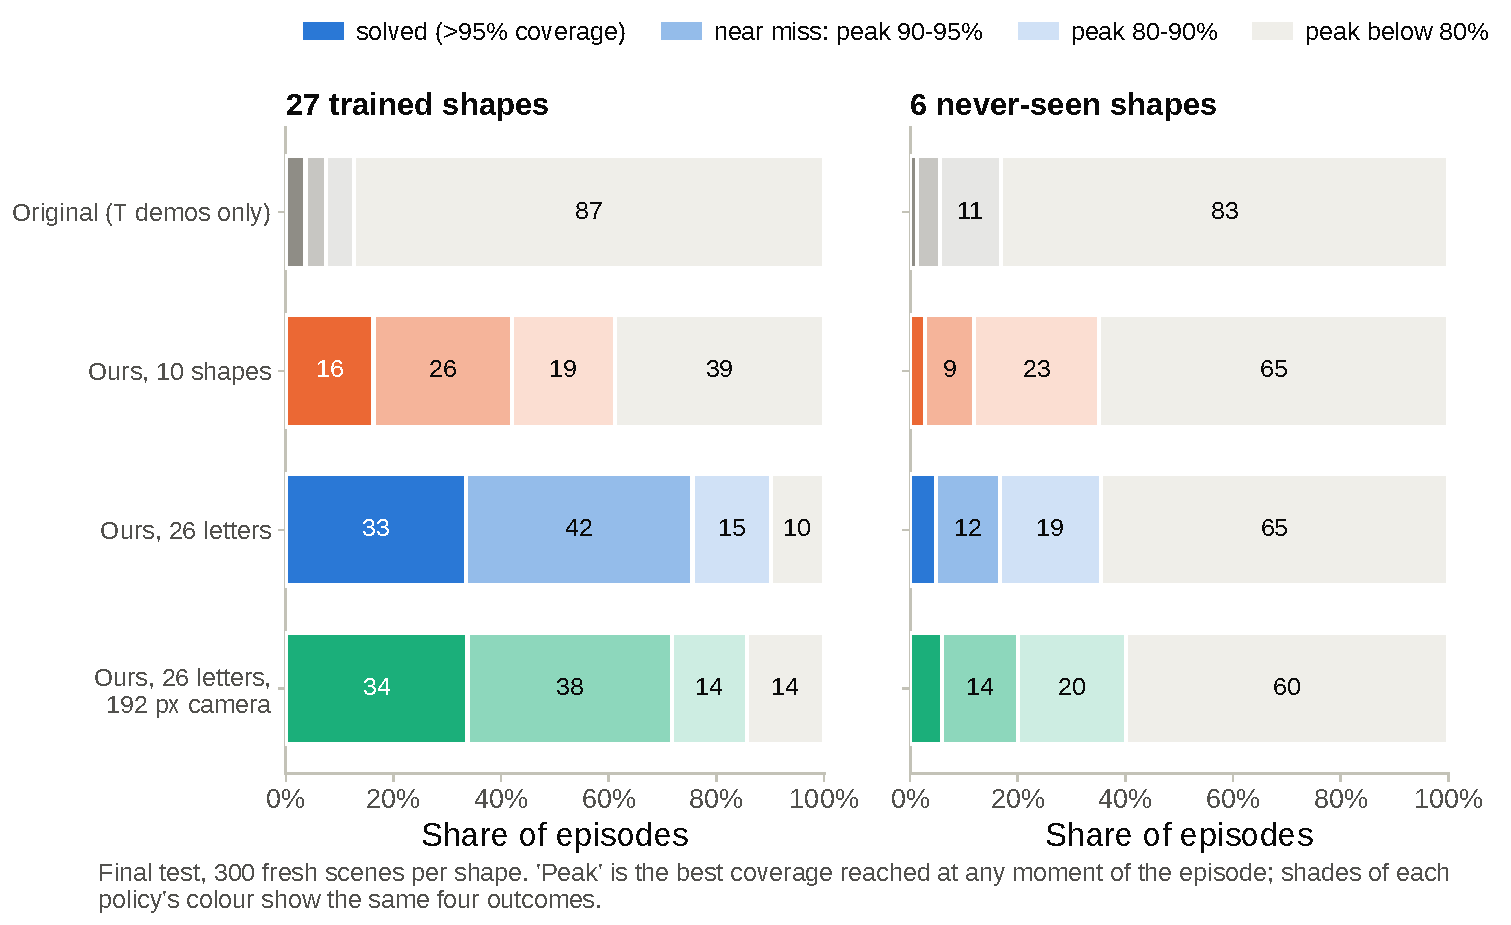
\includegraphics[width=\linewidth]{coverage_near_misses.pdf}
    \note{Blocks usually end close (91\% coverage at the best moment) but success needs 95\%.}
  \end{columns}
\end{frame}

\begin{frame}{What mattered}
  \begin{columns}[T]
    \column{0.33\textwidth}
    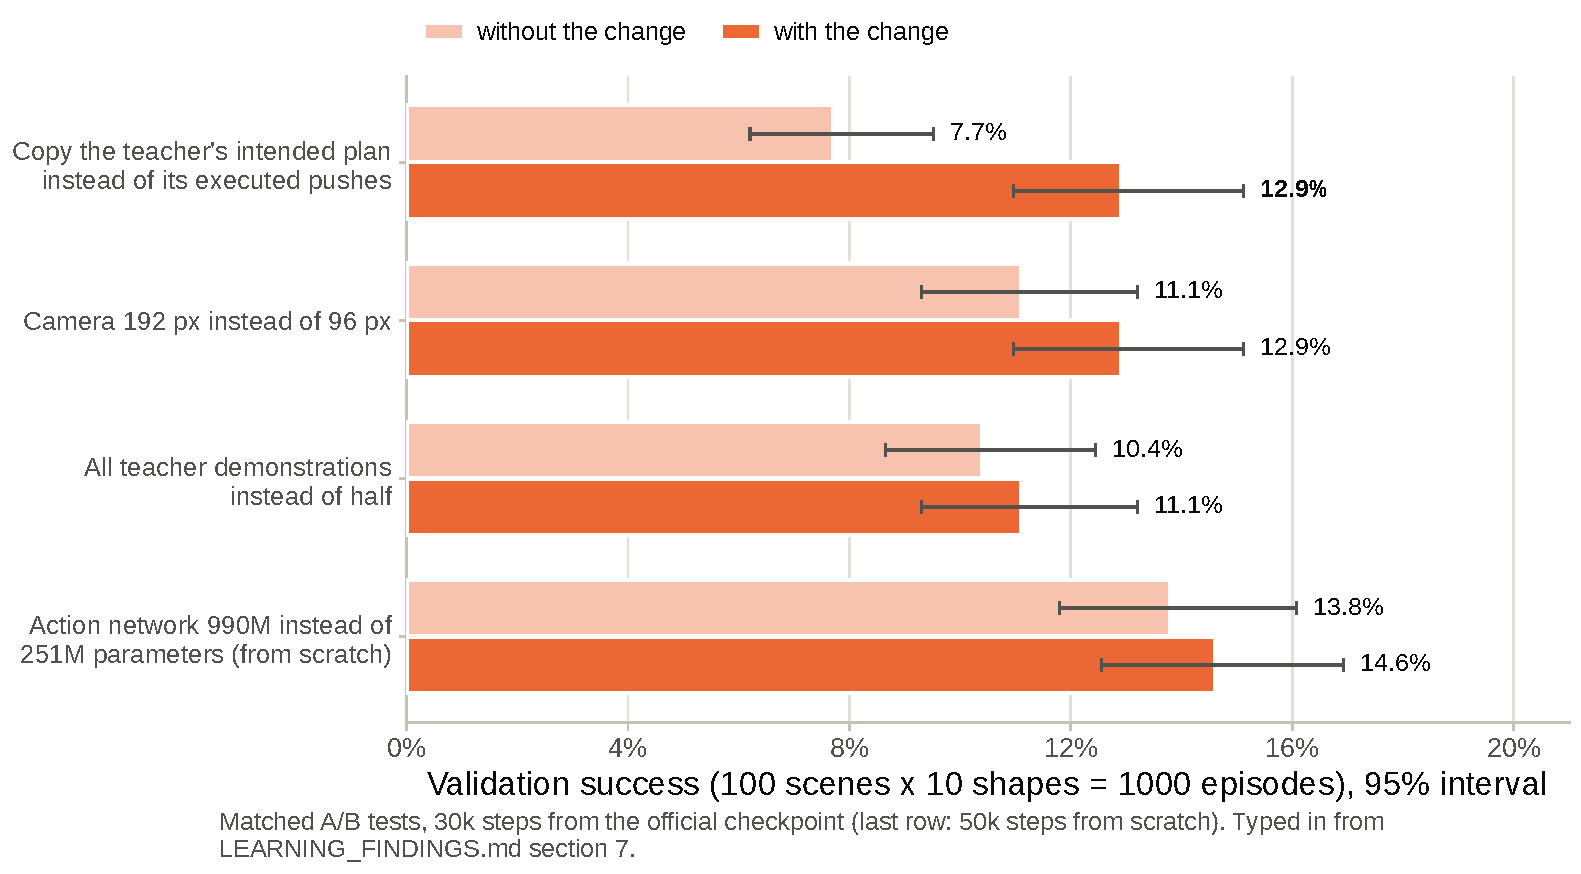
\includegraphics[width=\linewidth]{analysis_label_ab.pdf}
    \centering\note{Intended-plan labels}
    \column{0.33\textwidth}
    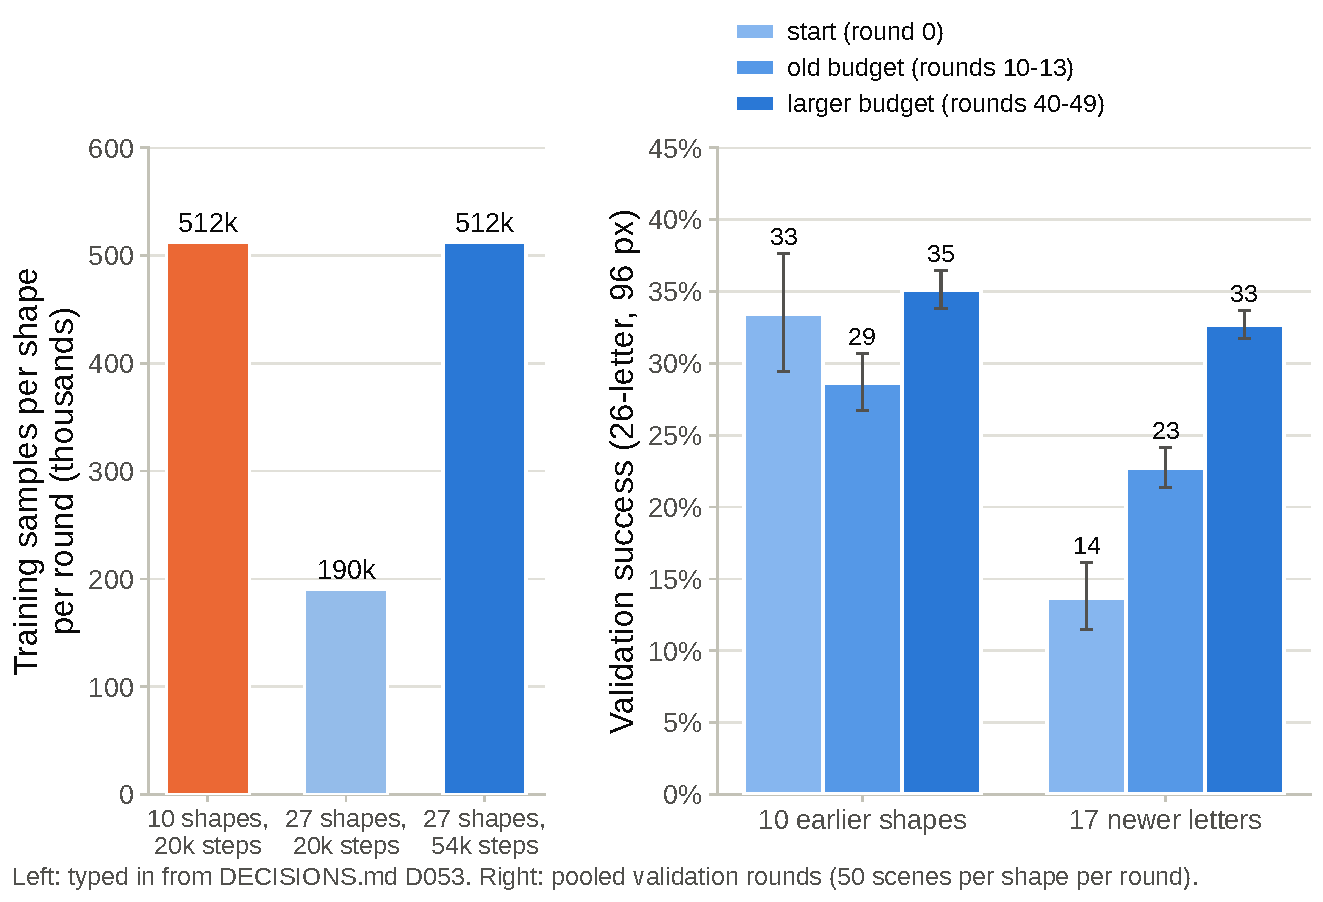
\includegraphics[width=\linewidth]{analysis_budget.pdf}
    \centering\note{Per-shape training budget}
    \column{0.33\textwidth}
    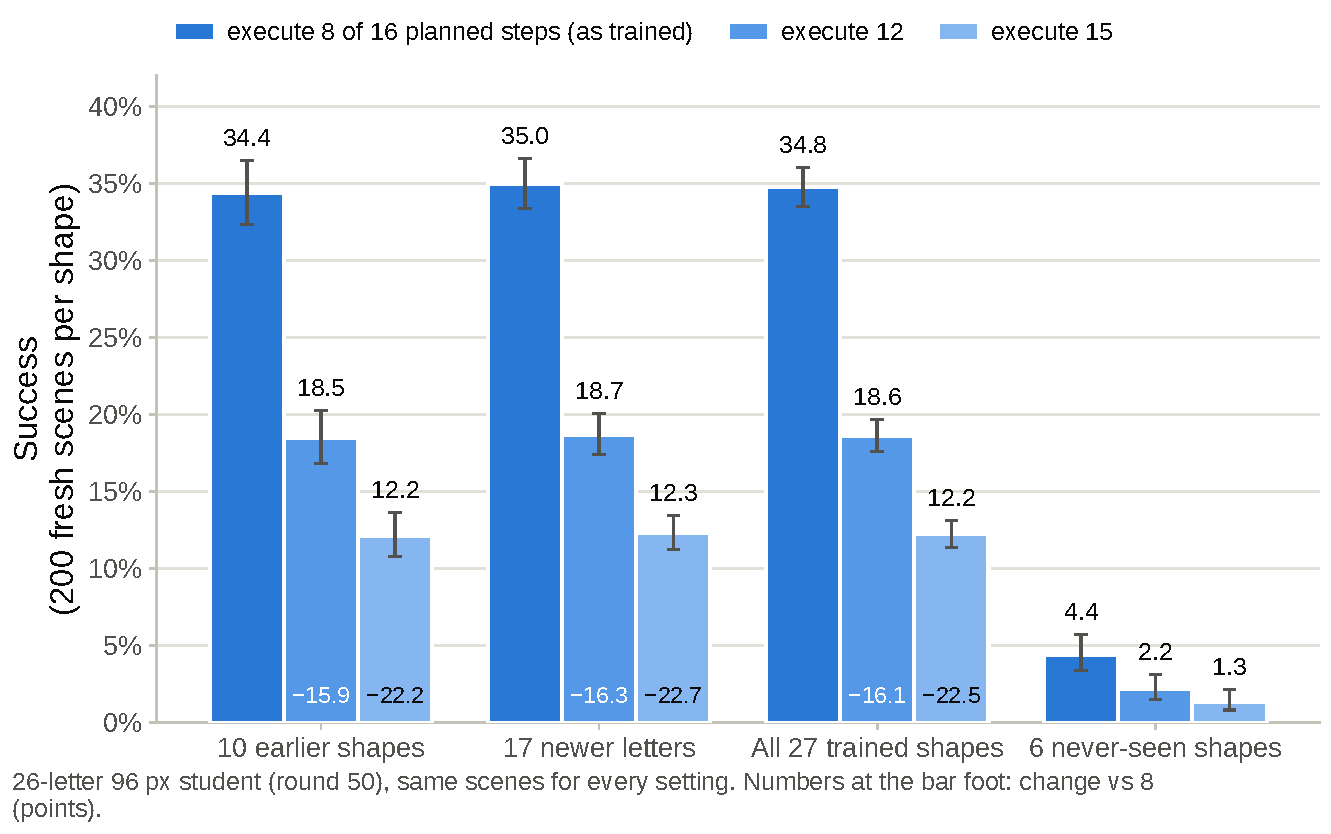
\includegraphics[width=\linewidth]{analysis_steps_executed.pdf}
    \centering\note{Executing 12 or 15 of 16 planned steps hurts}
  \end{columns}
\end{frame}

\begin{frame}{Limitations and disclosure}
  \begin{itemize}
    \item The teacher uses exact simulator state (training only); the tested policy is camera-only.
    \item Simulation only; no real robot.
    \item Final alignment is the open problem: one 96 px camera pixel is about 5 simulator pixels.
    \item T: 46.0\% $\rightarrow$ 40.7\% at 96 px in the final test (interval includes zero); 44.0\% for round 50.
    \item Machine-generated practice data on the target shapes: adaptation, not zero-shot transfer.
  \end{itemize}
\end{frame}

\begin{frame}{Conclusion}
  \begin{itemize}
    \item One camera policy for all 26 letters and near-T: \textbf{3.7\% $\rightarrow$ 33--35\%} on fresh scenes.
    \item No new human demonstrations: a privileged planner teaches, correction rounds fix the policy's own mistakes.
    \item Biggest levers: intended-plan labels and enough training per shape. RL fine-tuning did not work here.
    \item Next: sharper final alignment (camera resolution, last-mile corrections), real robot.
  \end{itemize}
  \vspace{4mm}
  \note{Code: github.com/Song-Mengfei/Tdyssey \quad Model: huggingface.co/LWZ19/tdyssey-pusht-26-letters}
\end{frame}

% ------------------------------------------------------------------ backup
\appendix
\begin{frame}{Backup: test protocol}
  \begin{itemize}
    \item Validation: 50 fixed scenes per shape (used for picking rounds). Final tests: unused seed pools, fixed before
          the run, all policies on the same scenes, 95\% intervals on paired differences.
    \item Success: more than 95\% of the goal covered within 300 controls. Standard 100-step DDPM sampling, 8 of 16
          planned steps executed.
  \end{itemize}
  \centering% Generated by presentation/scripts/make_figures.py from presentation/data/*.csv. Needs \usepackage{booktabs}.

\begin{tabular}{lrrrr}
\toprule
Shapes & Original & Ours, 10 shapes & Ours, 26 letters & Ours, 26 letters (192 px) \\
\midrule
10 earlier shapes & 9.3 & 33.0 & 33.7 & 34.2 \\
17 newer letters & 0.4 & 6.4 & 33.2 & 33.5 \\
All 27 trained shapes & 3.7 & 16.3 & \textbf{33.4} & \textbf{33.8} \\
6 never-seen shapes & 1.2 & 2.8 & 4.7 & 5.9 \\
\midrule
Change vs.\ original, all 27 trained shapes & -- & +12.6 [+11.8, +13.5] & +29.8 [+28.7, +30.9] & +30.1 [+29.0, +31.2] \\
Change vs.\ original, 6 never-seen shapes & -- & +1.6 [+0.7, +2.4] & +3.5 [+2.4, +4.6] & +4.7 [+3.5, +5.9] \\
Final coverage, 27 trained shapes & 0.35 & 0.63 & 0.82 & 0.81 \\
\bottomrule
\end{tabular}
% Success %; final test, 300 fresh scenes per shape, paired by scene; differences in points with 95% intervals.

\end{frame}

\begin{frame}{Backup: per-shape results}
  \centering\resizebox{!}{0.82\textheight}{% Generated by presentation/scripts/make_figures.py from presentation/data/*.csv. Needs \usepackage{booktabs}.

\begin{tabular}{lrrrr@{\hspace{1.5em}}lrrrr}
\toprule
Shape & Orig. & 10 sh. & 96 px & 192 px & Shape & Orig. & 10 sh. & 96 px & 192 px \\
\midrule
T & 46.0 & 42.7 & 40.7 & 38.3 & M & 0.7 & 1.7 & 38.7 & 37.7 \\
near-T & 37.3 & 32.0 & 29.0 & 32.3 & N & 0.3 & 0.3 & 38.7 & 41.7 \\
Y & 9.3 & 33.7 & 33.7 & 33.7 & O & 0.0 & 17.0 & 32.7 & 39.0 \\
D & 0.0 & 38.7 & 37.0 & 44.0 & Q & 0.0 & 6.3 & 28.7 & 22.0 \\
L & 0.0 & 30.3 & 35.0 & 34.0 & R & 0.3 & 10.7 & 37.3 & 28.0 \\
E & 0.0 & 23.3 & 31.7 & 28.0 & S & 1.7 & 3.3 & 39.0 & 33.7 \\
F & 0.0 & 28.3 & 30.0 & 29.3 & V & 0.0 & 5.0 & 30.7 & 27.3 \\
J & 0.0 & 21.3 & 21.3 & 19.0 & W & 0.0 & 12.0 & 40.0 & 39.0 \\
P & 0.0 & 46.7 & 48.7 & 51.3 & X & 0.0 & 2.3 & 38.0 & 36.7 \\
U & 0.0 & 33.3 & 30.3 & 32.3 & Z & 0.3 & 6.0 & 36.0 & 39.3 \\
A & 0.0 & 2.7 & 31.3 & 25.0 & digit 3 & 0.0 & 0.0 & 1.3 & 1.7 \\
B & 0.3 & 20.0 & 26.3 & 39.7 & digit 4 & 0.0 & 0.7 & 0.7 & 0.7 \\
C & 0.0 & 3.7 & 20.0 & 17.7 & digit 7 & 2.0 & 10.3 & 19.0 & 23.0 \\
G & 0.0 & 4.0 & 19.7 & 20.3 & plus & 0.7 & 1.3 & 0.3 & 0.3 \\
H & 0.0 & 4.3 & 40.7 & 45.7 & hash & 0.3 & 2.0 & 4.0 & 7.3 \\
I & 2.3 & 5.7 & 28.0 & 35.3 & arrow & 4.3 & 2.3 & 3.0 & 2.7 \\
K & 0.0 & 4.3 & 39.3 & 41.0 &  & & & &  \\
\bottomrule
\end{tabular}
% Success %, final test (D051), 300 fresh scenes per shape; 96 px and 192 px = the 27-shape students of rounds 44 and 2. Order: 10 earlier shapes, 17 newer letters, 6 never-seen shapes (digit 3 ... arrow).
}
\end{frame}

\begin{frame}{Backup: round 50 vs round 44, and the 192 px camera}
  \begin{columns}[T]
    \column{0.5\textwidth}
    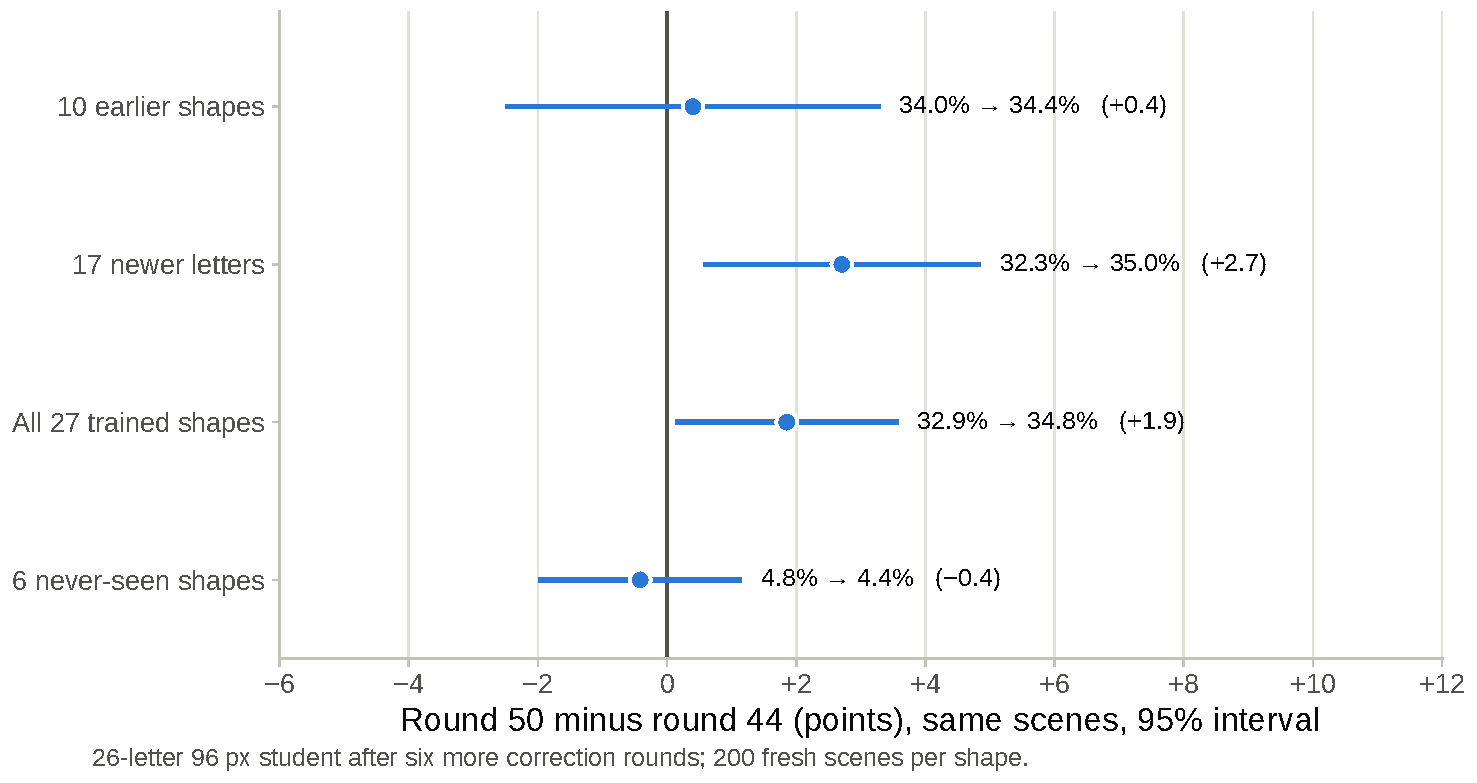
\includegraphics[width=\linewidth]{analysis_round50_vs_44.pdf}
    \column{0.5\textwidth}
    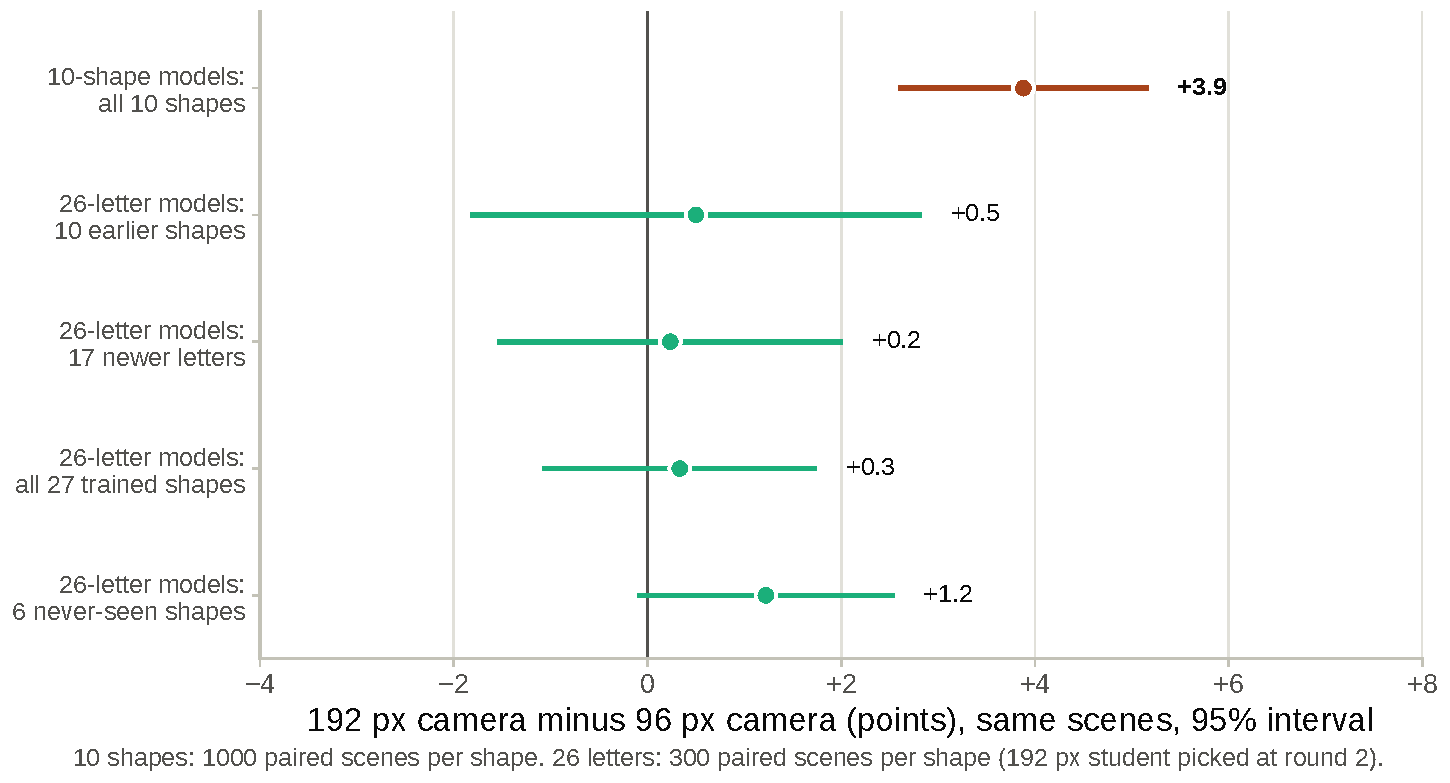
\includegraphics[width=\linewidth]{analysis_192_vs_96.pdf}
  \end{columns}
\end{frame}

\begin{frame}{Backup: T and near-T}
  \centering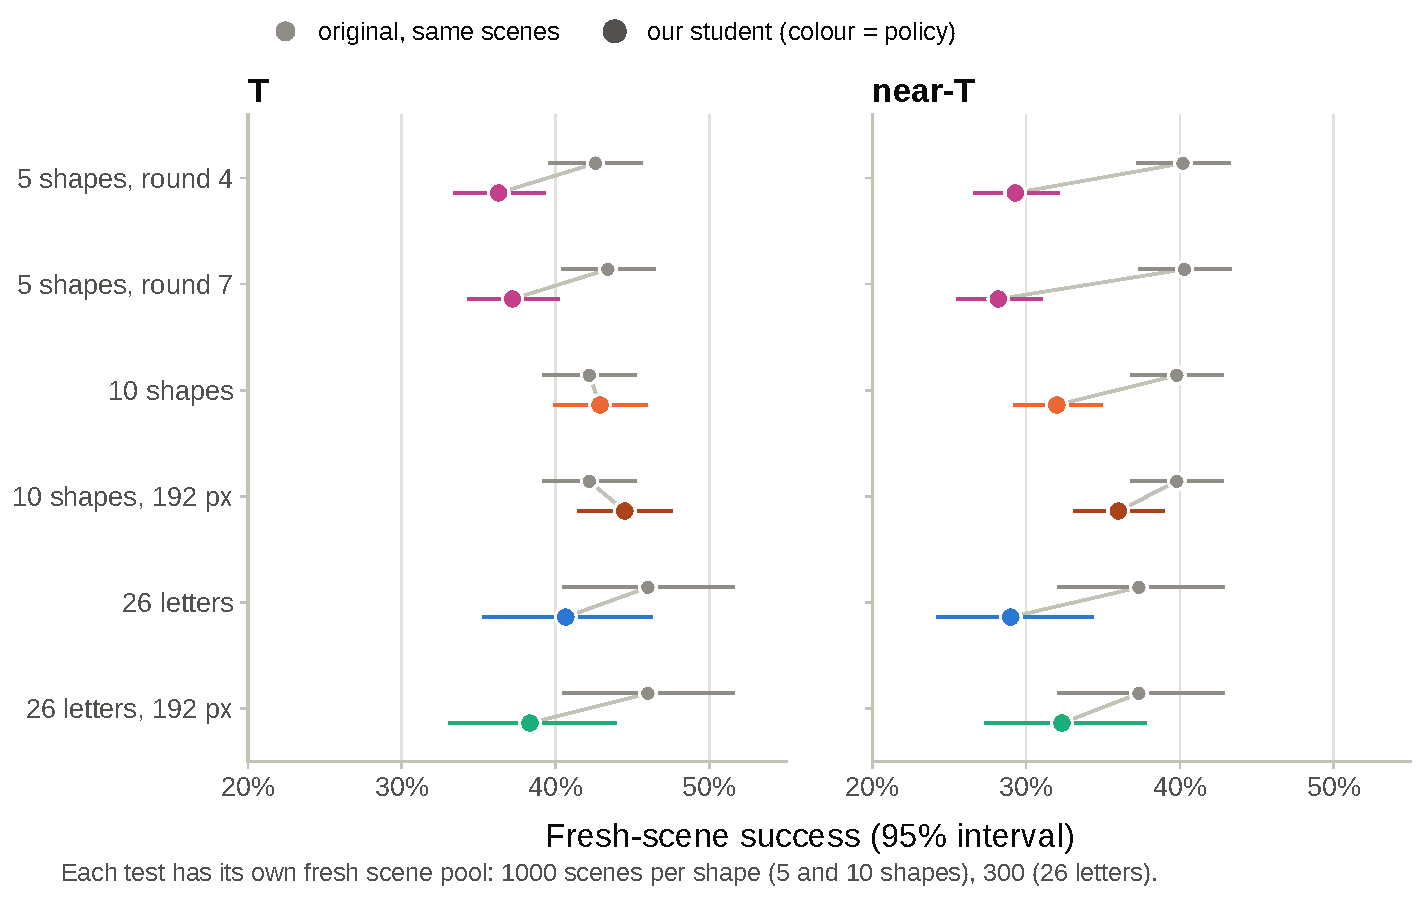
\includegraphics[width=0.8\textwidth]{analysis_t_tradeoff.pdf}
\end{frame}

\begin{frame}{Backup: ten shapes (1000 fresh scenes per shape)}
  \begin{columns}[T]
    \column{0.55\textwidth}
    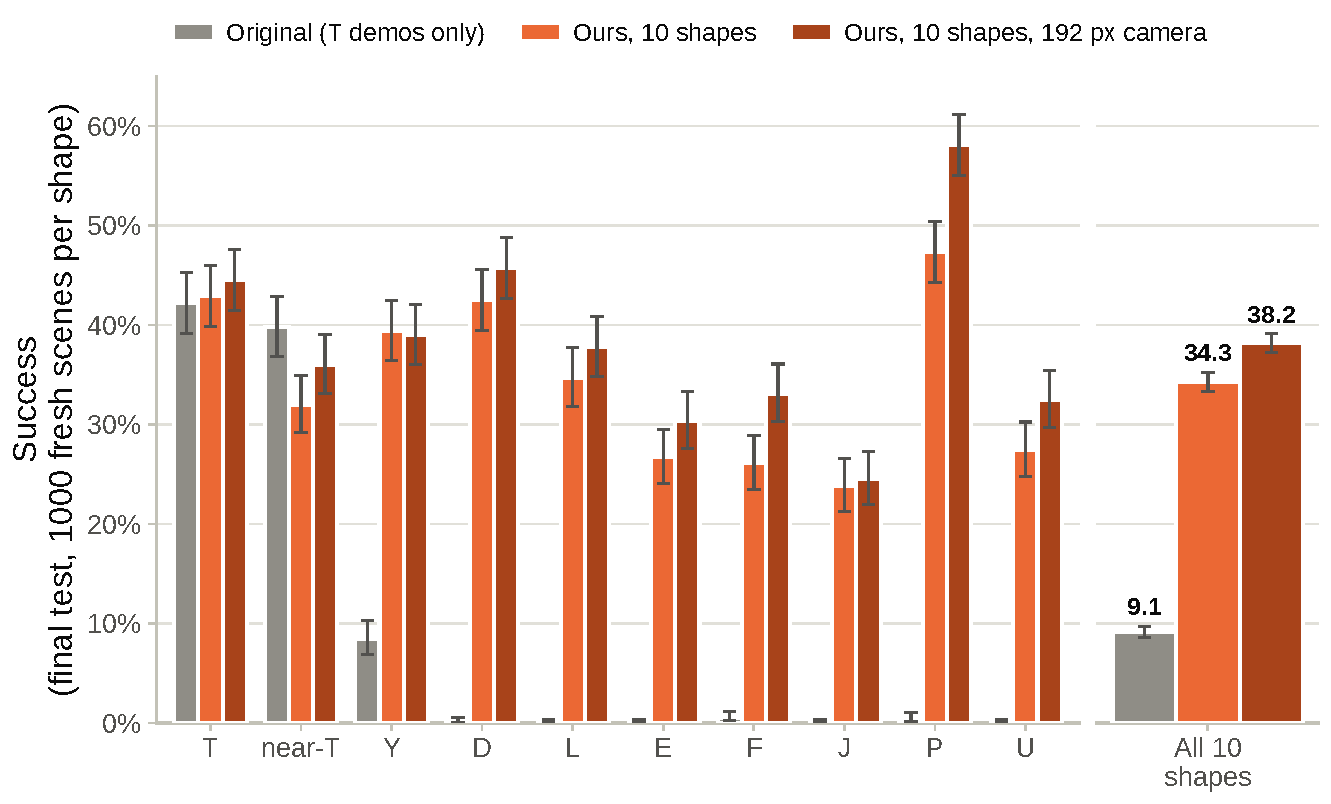
\includegraphics[width=\linewidth]{final_10shapes_bars.pdf}
    \column{0.43\textwidth}
    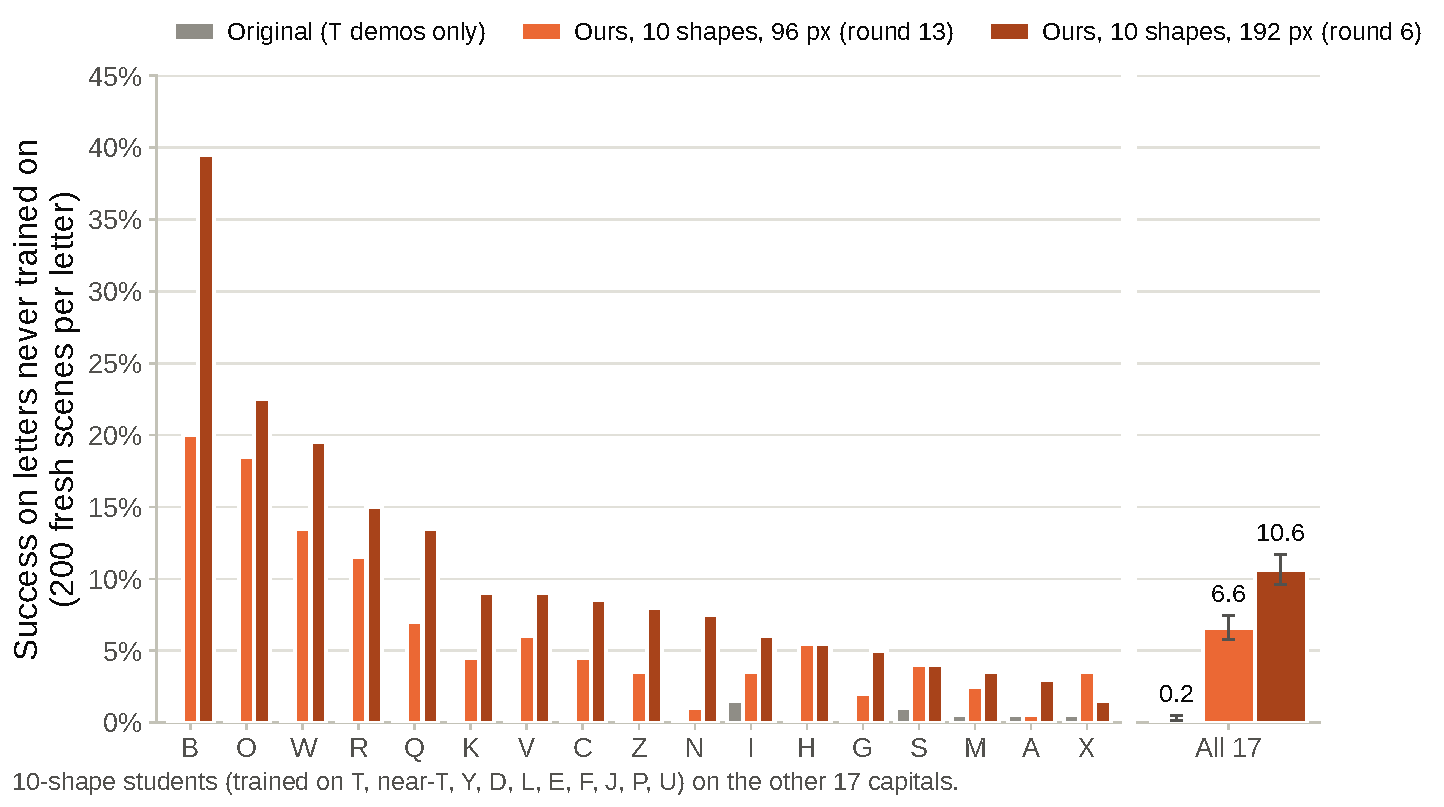
\includegraphics[width=\linewidth]{heldout_unseen_capitals.pdf}
    \note{The ten-shape models on the 17 capitals they never trained on.}
  \end{columns}
\end{frame}

\begin{frame}{Backup: the same scene through the project}
  \centering\video{progression_K.png}{../videos/progression/K_across_models.mp4}{0.72\textwidth}
\end{frame}

\begin{frame}{Backup: a never-seen shape solved (digit 7)}
  \centering\video{compare_digit7_scene2.png}{../videos/compare/digit7_scene2.mp4}{0.62\textwidth}\\
  \note{Digit 7 was never used in training; on fresh scenes it is solved 17--23\% of the time (original: 2\%).}
\end{frame}

\begin{frame}{Backup: teacher vs student per letter}
  \centering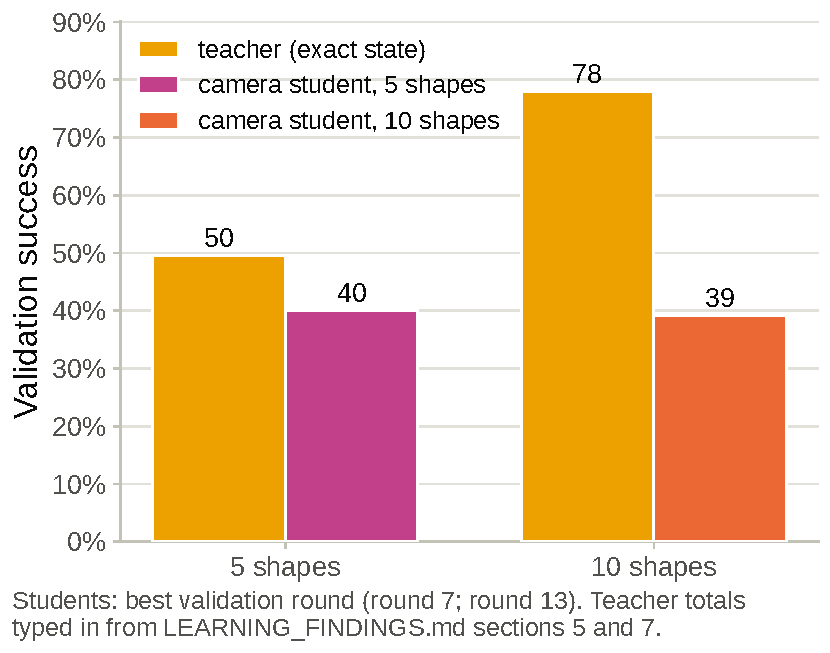
\includegraphics[width=0.85\textwidth]{method_teacher_gap.pdf}
\end{frame}

\end{document}
